\pdfoutput=1
\documentclass[11pt,a4paper]{article}
\usepackage{abhijit-research}
\renewcommand{\PaperCode}{P17}
\renewcommand{\PaperKind}{RESEARCH PAPER}
\renewcommand{\PaperVersion}{VERSION 1.0.1}
\renewcommand{\PaperDate}{AUGUST 2026}
\renewcommand{\PaperTitle}{Prime-Indexed Return Sectors}
\renewcommand{\PaperSubtitle}{The Thirty-Six-Relation Closure of a Nine-State Carrier}
\renewcommand{\PaperFullTitle}{Prime-Indexed Return Sectors and the Thirty-Six-Relation Closure of a Nine-State Carrier}
\renewcommand{\PaperShortTitle}{Prime-Indexed Return Sectors}
\renewcommand{\PaperKeywords}{prime arity; predictive quotient; occurrence identity; relation lattice; recurrence exponent; finite spectral labels}
\renewcommand{\PaperClassification}{The carrier, involution, 36-cell decomposition, reporter-closure, critical-return, occupation-state, and finite predictive-quotient results are exact. The term quantum number is used first in its mathematical spectral-label sense. A physical realization requires independently specified observables and dynamics.}
\renewcommand{\PaperCitation}{Singh, Abhijit. 2026. \textit{Prime-Indexed Return Sectors and the Thirty-Six-Relation Closure of a Nine-State Carrier}. Research manuscript, version 1.0.1.}
\begin{document}
\MakeResearchTitle
\MakeResearchContents
\MakeResearchAbstract{%
A finite observer-closure theorem is developed from an occurrence-sensitive prime relation. The two appearances of a prime in $p\cdot1=p$ have equal numerical value but different source and return roles. A value-only reporter turns their directed relation into a self-loop; an occurrence-sensitive reporter retains a period-two return. On the decimal terminal carrier $\mathbb Z_{10}$, the zero and unit are terminal roles, while the eight nonterminal indices form four prime/composite pairs under the fixed-point-free affine involution $\sigma(d)=1-d\pmod {10}$. Removing the zero terminal leaves nine active states. Their complete unordered relation frontier contains $\binom92=36$ cells and decomposes exactly into eight unit relations, four return-sector relations, and twenty-four transverse relations. The four prime labels $2,3,5,7$ are independently selected by transparent arity. Together with a side label they form complete commuting spectral coordinates on the finite carrier; the four return planes commute inside the 36-dimensional antisymmetric relation space. The finite prime/composite reporter is then refined by prime-occupation coordinates: $6$ is squarefree coupling, whereas $4,8,9$ are repeated-prime states. The resulting static five-class reporter is proved insufficient under arbitrary prime multiplication, and the all-scale predictive quotient is the finite prime-support address plus one absorbing repeated-prime state. The theorem is related to the earlier nine-transformation, thirty-six-witness closure, recurrence selection, quotient closure, harmonic realization, and arithmetic completion without identifying merely isomorphic carriers as the same physical system.
}

\section{Occurrence-sensitive prime relation}
For a prime $p$, ordinary arithmetic writes
\begin{equation}
p\cdot1=p.
\end{equation}
The two tokens labelled $p$ have one value but two roles. Write
\begin{equation}
p_{\rm source}\cdot1_{\rm unit}=p_{\rm return},
\qquad
v(p_{\rm source})=v(p_{\rm return})=p,
\qquad
p_{\rm source}\ne_{\rm occ}p_{\rm return}.
\end{equation}
The fourth component is the relation-establishing operation and its retained mark. It is not another numerical factor.

\begin{proposition}[Factor-complete prime triad]
For an integer $n>1$, the reduced triad $(n_{\rm source},1_{\rm unit},n_{\rm return})$ contains every positive factor relation of $n$ if and only if $n$ is prime.
\end{proposition}
\begin{proof}
If $n$ is prime, every positive factor pair is $(1,n)$ or $(n,1)$. If $n$ is composite, some $1<a,b<n$ satisfy $ab=n$, and that relation is absent from the reduced triad.
\end{proof}

The proposition is deliberately modest. Its significance lies in reporter design: a terminal primality report is complete for the declared positive-factor query, while a generative prime-power or multiplication query requires occurrence and multiplicity coordinates.

\section{Terminal lattice and affine return}
Let
\begin{equation}
D=\mathbb Z_{10},\qquad T=\{0,1\},\qquad I=\{2,3,4,5,6,7,8,9\},\qquad A=D\setminus\{0\}.
\end{equation}
Define
\begin{equation}
\sigma(d)=1-d\pmod {10}.
\end{equation}
It has no fixed point on $D$ and has the five orbits
\begin{equation}
(0,1),\ (2,9),\ (3,8),\ (4,7),\ (5,6).
\end{equation}
The restriction to $I$ pairs every prime index with one composite index. Put
\begin{equation}
P=\{2,3,5,7\},\qquad C=\{4,6,8,9\}.
\end{equation}
For $q\in P$, define $\bar q=\sigma(q)$ and encode the interior as
\begin{equation}
I\cong P\times\{+,-\},\qquad(q,+)=q,\qquad(q,-)=\bar q.
\end{equation}
Then
\begin{equation}
\sigma(q,\varepsilon)=(q,-\varepsilon).
\end{equation}

\begin{figure}[H]
\centering
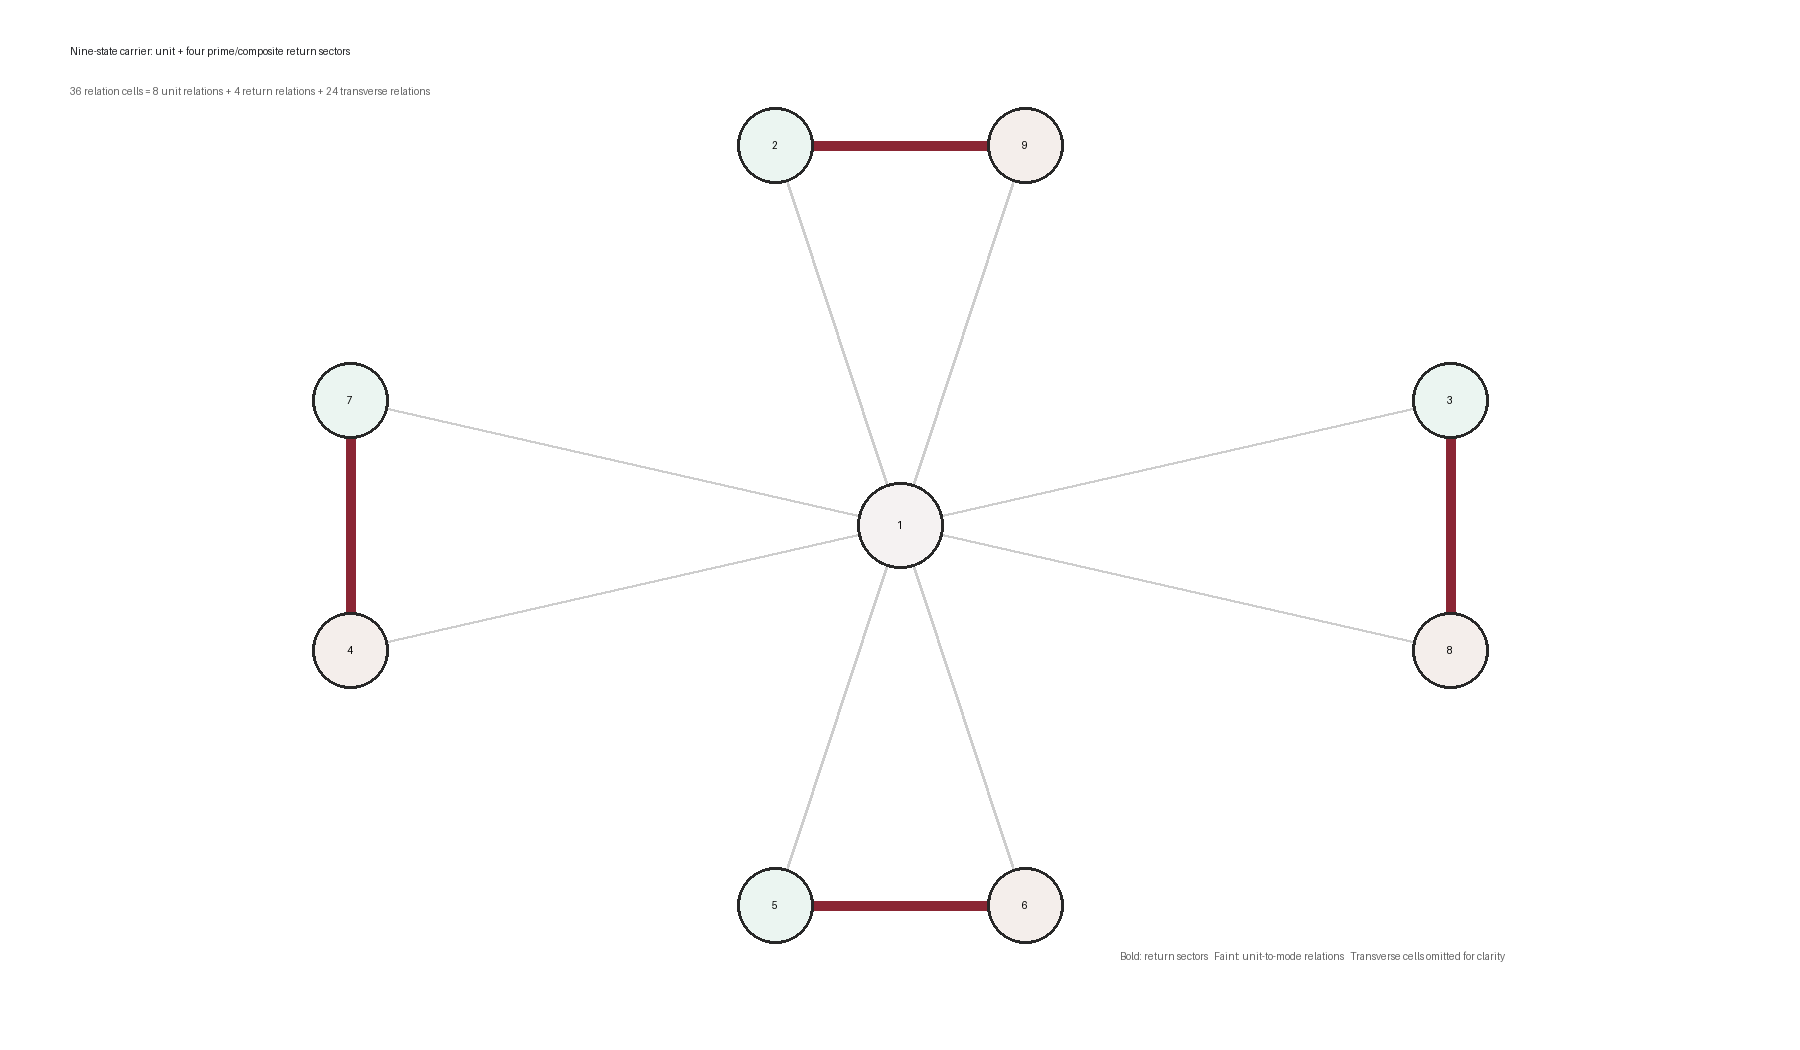
\includegraphics[width=.92\linewidth]{figures/nine_state_relation_frontier.png}
\caption{The active nine-state carrier. Bold edges are the four prime/composite return sectors. The eight unit relations are shown faintly; the twenty-four transverse relation cells complete the rank-two frontier.}
\end{figure}

\section{Thirty-six-relation closure theorem}
Let
\begin{equation}
\mathcal R_2(A)=\{\{x,y\}:x,y\in A,\ x\ne y\}
\end{equation}
be the complete unordered pair-relation frontier.

\begin{theorem}[Nine-state, thirty-six-relation closure]
The active carrier has nine states and
\begin{equation}
|\mathcal R_2(A)|=\binom92=36.
\end{equation}
The frontier decomposes canonically as
\begin{equation}
\boxed{36=8_{\rm unit}+4_{\rm return}+24_{\rm transverse}}.
\end{equation}
The four return relations are $\{q,\bar q\}$ for $q\in P$. The transverse relations connect different return sectors.
\end{theorem}
\begin{proof}
There are eight relations from the unit state $1$ to the eight interior states. There are four within-sector relations. For each of the $\binom42=6$ pairs of two-element sectors, there are $2\cdot2=4$ cross-sector relations, giving $24$. The classes are disjoint and exhaustive.
\end{proof}

This is more accurately a 36-cell rank-two relation layer than a 36-state carrier. Each cell is one possible distinction between two of the nine active states.

\section{Observer quotient and critical recurrence}
Define the side-forgetting reporter
\begin{equation}
U(1)=1,\qquad U(q,\varepsilon)=q.
\end{equation}
Let the return map be
\begin{equation}
R(1)=1,\qquad R(q,\varepsilon)=(q,-\varepsilon).
\end{equation}
Then $U\circ R=U$, although $R$ has period two on every interior sector.

\begin{theorem}[Apparent halt versus retained return]
For every $q\in P$, the complete state alternates
\begin{equation}
(q,+)\leftrightarrow(q,-),
\end{equation}
while the quotient report remains constant. If $r_q=e_{q,+}-e_{q,-}$ and the residual propagator is the return flip, then
\begin{equation}
Rr_q=-r_q,\qquad \|R^nr_q\|=\|r_q\|,
\end{equation}
and therefore $\chi(r_q)=0$ for every linear intrinsic clock.
\end{theorem}
\begin{proof}
The first statement is immediate. The residual changes sign under the swap and therefore has constant norm. Its logarithmic growth rate is zero.
\end{proof}

Thus a reporter that stops when its visible output repeats records a halt; a reporter that preserves occurrence sees recurrence. The equality $U(r_q)=0$ is report-level erasure, not dynamical assimilation. If an admitted future distinguishes the two sides, the complete-behaviour closure criterion forces the refined state $(q,\varepsilon)$.

\section{Prime selection and finite spectral labels}
Transparent arity is defined by
\begin{equation}
\binom qk\equiv0\pmod q\qquad(0<k<q).
\end{equation}
The transparent arities are exactly the primes. Hence $2,3,5,7$ are not selected by the decimal drawing; they are the first four transparent nonterminal arities in the finite carrier.

Let
\begin{equation}
\mathcal H_A=\mathbb C|1,0\rangle\oplus\bigoplus_{q\in P,\ \varepsilon=\pm1}\mathbb C|q,\varepsilon\rangle.
\end{equation}
Define commuting diagonal operators
\begin{equation}
\widehat Q|q,\varepsilon\rangle=q|q,\varepsilon\rangle,
\qquad
\widehat S|q,\varepsilon\rangle=\varepsilon|q,\varepsilon\rangle.
\end{equation}
The pair $(Q,S)$ is a complete finite label. In this exact mathematical sense it is a system of quantum numbers: joint eigenvalues of commuting operators. Physical quantum numbers require a specified physical observable and transition law; the finite labelling theorem alone does not provide them.

The full oriented pair-relation space is
\begin{equation}
\bigwedge^2\mathbb R^9\cong\mathfrak{so}(9),\qquad \dim\bigwedge^2\mathbb R^9=36.
\end{equation}
For each return sector define
\begin{equation}
J_q=E_{q,\bar q}-E_{\bar q,q}.
\end{equation}
The four $J_q$ act on disjoint two-planes and therefore commute. This is a finite relation representation, not a derived physical $SO(9)$ gauge theory.

\section{Prime-occupation refinement}
Unique factorisation gives commuting occupation labels
\begin{equation}
N_p|d\rangle=v_p(d)|d\rangle,\qquad p\in\{2,3,5,7\}.
\end{equation}
The finite states are therefore separated as follows.
\begin{center}
\begin{tabular}{ccl}
\toprule
index&$(n_2,n_3,n_5,n_7)$&type\\\midrule
$1$&$(0,0,0,0)$&unit\\
$2,3,5,7$&one unit occupation&primitive prime mode\\
$6$&$(1,1,0,0)$&squarefree coupling\\
$4,8,9$&a repeated occupation&repeated-prime state\\
\bottomrule
\end{tabular}
\end{center}
Accordingly the coarsest terminal-resolved static M\"obius reporter on the digit carrier has five classes
\begin{equation}
\{0\},\quad\{1\},\quad\{2,3,5,7\},\quad\{6\},\quad\{4,8,9\}.
\end{equation}

\begin{theorem}[Static five-class false closure]
The five-class reporter is not a continuation congruence when multiplication by arbitrary primes is admitted. The coarsest all-prime predictive quotient for future M\"obius reports consists of one state for every finite squarefree prime-support set and one absorbing repeated-prime state.
\end{theorem}
\begin{proof}
The primes $2$ and $3$ share the static prime class. Multiplication by $2$ sends them to $4$ and $6$, whose M\"obius reports are $0$ and $+1$. Hence the static quotient fails. For the full quotient, represent a squarefree integer by its finite prime support and every nonsquarefree integer by $\dagger$. Multiplication by $p$ adjoins $p$ when absent and sends the state to $\dagger$ when present; $\dagger$ is absorbing. Distinct supports are future-distinguishable: choose a prime in their symmetric difference and multiply by it. One state repeats that prime and the other does not. Therefore no coarser reporter preserves every prime-multiplication future.
\end{proof}

This theorem locates the limit of the finite 36-cell picture. It is a complete finite relation frontier, but the all-prime predictive state is necessarily unbounded in the number of possible support addresses.

\section{Harmonic realization and scale boundary}
For any positive fundamental $f_0$, define
\begin{equation}
f_d=f_0d,\qquad d=0,1,\ldots,9.
\end{equation}
At $f_0=111\,\mathrm{Hz}$ the coefficients appear as decimal repdigits. The prime-indexed and composite-indexed modes are
\begin{equation}
111\{2,3,5,7\}\quad\text{and}\quad111\{4,6,8,9\}.
\end{equation}
Their indicator sequences are affine reflections and have identical cyclic Fourier magnitudes. Equal-amplitude multitone realizations are equal-energy and orthogonal over the common period $1/f_0$. The structure is invariant under positive rescaling; therefore it does not select $111\,\mathrm{Hz}$ as a natural constant, nor does the arithmetic alone imply a biological or therapeutic effect.

\section{Relation to the earlier nine-transformation closure}
A separate finite construction generated nine causally distinguishable whole-carrier transformations and an exact pairwise witness for each of their $36$ unordered pairs. Both systems therefore have a complete relation frontier isomorphic to the edge set of $K_9$.

\begin{proposition}[Relation-frontier isomorphism and its limit]
Any bijection between two nine-element carriers induces an isomorphism of their 36-cell unordered relation frontiers. It preserves operational meaning only when it also intertwines the declared continuations and source provenance.
\end{proposition}
\begin{proof}
A bijection maps unordered pairs bijectively. Graph isomorphism alone says nothing about continuation responses. Those are preserved exactly when the vertex map commutes with the relevant operations and reporters.
\end{proof}

Thus the two nine-state constructions reinforce the role of complete pairwise distinction, but combinatorial isomorphism is not used as evidence that their vertices or physical meanings are identical.

\section{Integration with the wider programme}
The theorem joins the earlier work in one precise chain:
\begin{equation}
\text{occurrence}\to\text{relation}\to\text{report}\to\text{future test}\to\text{assimilation, retention, or promotion}.
\end{equation}
The prime triad supplies the smallest occurrence-sensitive example. The 36-cell frontier enumerates every pair distinction on the nine active states. The recurrence exponent distinguishes genuine assimilation from report-level erasure. Prime transparency selects the sector labels. Occupation coordinates refine the composite class. The all-prime quotient shows that a finite reporter can be exact for one envelope and false for a larger one. The adaptive-system architecture turns this sequence into an executable repair protocol.

\section{Verification and claim boundary}
The ancillary verifier checks the affine involution, the four prime/composite pairs, the $8+4+24$ relation decomposition, commutation of the four return-plane generators, Fourier-magnitude equality, the static five-class counterexample, and deterministic prime-support updates.

The paper does not claim that nature has exactly nine states, that $SO(9)$ is a physical gauge group, that $2,3,5,7$ are measured physical quantum numbers, that $111\,\mathrm{Hz}$ is fundamental, or that the finite carrier proves the Riemann Hypothesis. It establishes the finite theorem, the exact predictive-closure correction, and the conditions required for a physical realization.


\begin{thebibliography}{99}
\bibitem{perspectives} A. Singh, Future-Complete Quotients and Recursive Distinction, research manuscript, 2026.
\bibitem{recurrence} A. Singh, Recurrence Exponents, Accessibility Growth, and Predictive-State Promotion, research manuscript, 2026.
\bibitem{arity} A. Singh, Arity-Indexed Refinement Posets, Forced Inverses, and Rotational Root Geometry, research manuscript, 2026.
\bibitem{capacity} A. Singh, Capacity Complexes, One-Bit Persistence, and Operator-Ideal Criticality, research manuscript, 2026.
\bibitem{rh} A. Singh, Critical Capacity Completion and Equivalent Forms of the Riemann Hypothesis, research manuscript, 2026.
\bibitem{genesis} A. Singh, Provenance-Preserving Representation Genesis in Finite Deterministic Systems, research manuscript, 2026.
\bibitem{crossprojection} A. Singh, Distinction, Perspective, and Emergent Law: Complete Research Record, 2026.
\end{thebibliography}
\end{document}
